%!TEX program = xelatex
\documentclass[10pt]{beamer}
\usepackage{graphicx}
\usepackage{booktabs}
\linespread{1.11}
\usepackage{tikz}
\tikzset{global scale/.style={
    scale=#1,
    every node/.style={scale=#1}
  }
}
\setcounter{tocdepth}{1}

\usetheme[menuwidth={0.7\paperwidth}]{erlangen}
\setbeamercovered{transparent=20}
\setbeamerfont{frametitle}{series=\bfseries}
\usepackage{hyperref}
\hypersetup{colorlinks=false,
            colorlinks=black,
            pdfborder=100,
            citecolor=black}


\setbeamerfont{block title}{series=\bfseries}
\usepackage{graphicx}


\usepackage[no-math,cm-default]{fontspec}
\setmainfont{Minion Pro}
\setsansfont[BoldFont={Myriad Pro Semibold}]{Myriad Pro}
\setmonofont{Courier New}
\usepackage{xeCJK}
\setCJKmainfont[BoldFont={方正黑体简体},ItalicFont={楷体}]{宋体}
\setCJKsansfont[BoldFont={方正黑体简体}]{方正中等线简体}
\setCJKmonofont{方正中等线简体}
\XeTeXlinebreaklocale "zh"
\XeTeXlinebreakskip = 0pt plus 1pt

\usefonttheme[onlymath]{serif}
\usepackage[noamssymbols]{mtpro2}

% \renewcommand\contentsname{目录}
\setbeamertemplate{itemize items}{\raisebox{0.15ex}{\small$\bullet$}}

\begin{document}
\title{Migrants\rq{} Remittance and Happiness}
\subtitle{Evidence from Shanghai (China)}
\author{DENG Dongsheng}
\date{\today}
% \institute{The School of Economics\\
  % \vspace{-0.2em}{\small Fudan University} }

\begin{frame}[plain]
  \titlepage
\end{frame}


\begin{frame}{Table of Contents}
  \tableofcontents
\end{frame}


\section{Introduction}

\begin{frame}[c]\frametitle{Migration to Beijing}
\begin{center}
   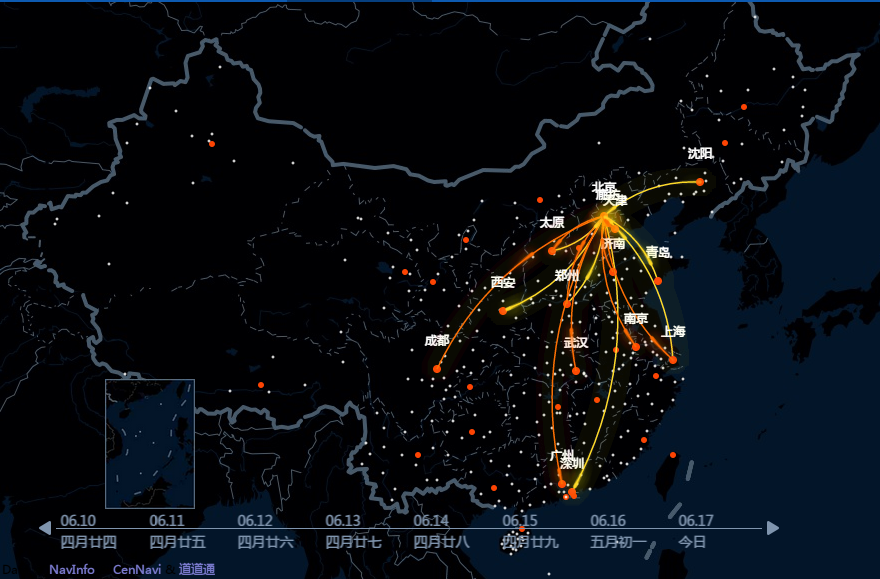
\includegraphics[width=0.9\textwidth]{baidu.png}
\end{center}

\end{frame}

\begin{frame}[c]\frametitle{Migration to Shanghai}
\begin{center}
   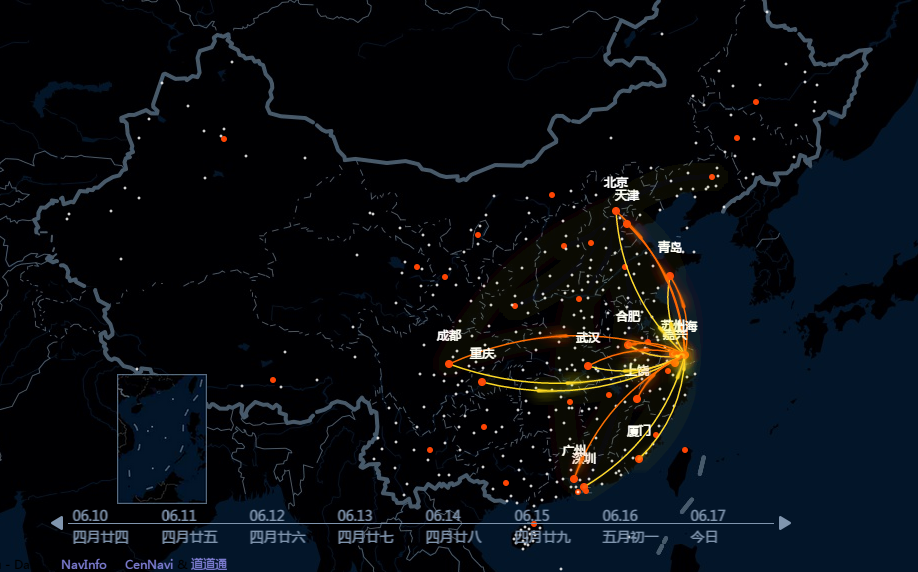
\includegraphics[width=0.9\textwidth]{baidu3.png}
\end{center}

\end{frame}

\begin{frame}[c]\frametitle{Migration Flow Data}

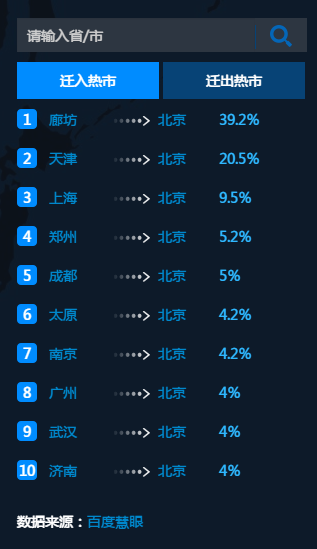
\includegraphics[height=0.8\textheight]{baidu2.png}
\hfill
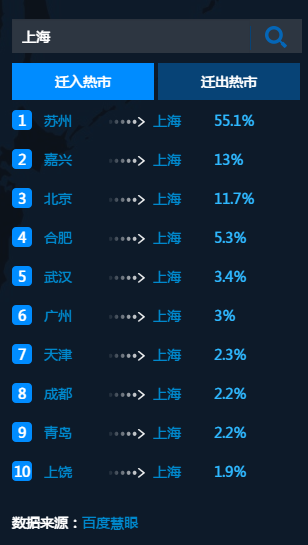
\includegraphics[height=0.8\textheight]{baidu4.png}


\end{frame}

\begin{frame}[c]\frametitle{Introduction}
\begin{itemize}
    \item The migrants have much contribution in the process of
    China\rq{}s economic development, they cannot fullly share the achievement of development;
    \item Constrained by the household registration system, some family members are left behind;
    \item Migrants will send some money back to support the home family;
    \item Increasing analysis the welfare of the "silent group";
    \item This paper is to understand the relationship between the remittance and wellbeing (happiness).
\end{itemize}

\end{frame}

\section{Related Literature}

\begin{frame}[c]\frametitle{Scope of Remittance (Luo 2007)}
\alert{Remittance}: all the net source transfer including
\begin{itemize}
    \item Money or commodities send back to the home family through post office or bank + money bring back.
    \item Money or commodities deliver to the home family by acquaintance.
    \item All the payment during the home family visit.
    \item All the payment during the home family\rq{}s visit.
    \item Donation to hometown.
\end{itemize}

\end{frame}

\begin{frame}[c]\frametitle{Evidence from International Migration(WB 2013)}

\begin{itemize}
    \item Remittances to developing countries were an estimated \$404 billion (+3.3\%);
    \item Including those to high-income countries \$542 billion;
    \item $\gamma$(developing country) = 2\%, $\gamma$(low income country) = 6\%, where $\gamma \equiv \text{Remittance}/\text{GDP}$;
    \item Tajikistan (52\%), Kyrgyz Republic (31\%);
    \item Nepal and Moldova (both 25\%);
    \item Samoa and Lesotho (both 23\%).
\end{itemize}

\end{frame}

\begin{frame}[c]\frametitle{Characteristics of Chinese Migants (Li 2004)}
\begin{enumerate}
    \item Highest ratio (remittance/home income);
    \item Altruism by nature?
    \item Thrift (consume as less as possible)?
    \item Remittance and saving are similar?
    \item Lower income region, higher remittance
    \item Remittance and migrant has narrow the income gap btw the poor region and the rich, while deepen the income gap btw the "migrant" area and "non-migrant" area.
\end{enumerate}
\end{frame}



\begin{frame}[c]\frametitle{Motivation of Remittance (Lucas \& Stark 1985)}

\begin{enumerate}
    \item Pure Altruism;
    \begin{itemize}
        \item spending money on other people have a more positive impact on happiness than spending money on oneself (from Dunn, Aknin, Norton 2013).
    \end{itemize}
    \item Pure Self-Interest;
    \begin{itemize}
        \item aspiration to inherit;
        \item ensure home careful maintenance of their assets;
        \item the intent to return home, fixed assets or social assets (relationship) investment.
    \end{itemize}
    \item Tempered Altruism or Enlightened Self-Interest;
    \begin{itemize}
        \item viewing remittances as part of an intertemporal, mutually beneficial contractual arrangement between migrant and home.
    \end{itemize}
\end{enumerate}
\end{frame}

\begin{frame}[t]\frametitle{Chinese Social Behavior and Relationship Network \par (Li \& Luo 2013)}

\begin{itemize}
    \item Rational behavior and  instrumental reductionism (Economics)
    \item Mixed sources of action (Social Network Theory):
    \begin{itemize}
        \item not only a rational choice based on pure self-interest,
        \item includes the of trusted cooperation and obedience of power(status).
    \end{itemize}
    \item Trust, unity, cooperation, obedience is the opposite of the interests of the individual, at least, is the opposite short-term personal interests;
    \item Rational calculation theory cannot fully explain the economic and social phenomenon.
    \item The interpretation of the social network theory framework is not based on a single interest motivation this most fragile foundations, but emphasize social behavior motivation.
\end{itemize}

\end{frame}

\begin{frame}[c]\frametitle{Mechanism}

\begin{center}
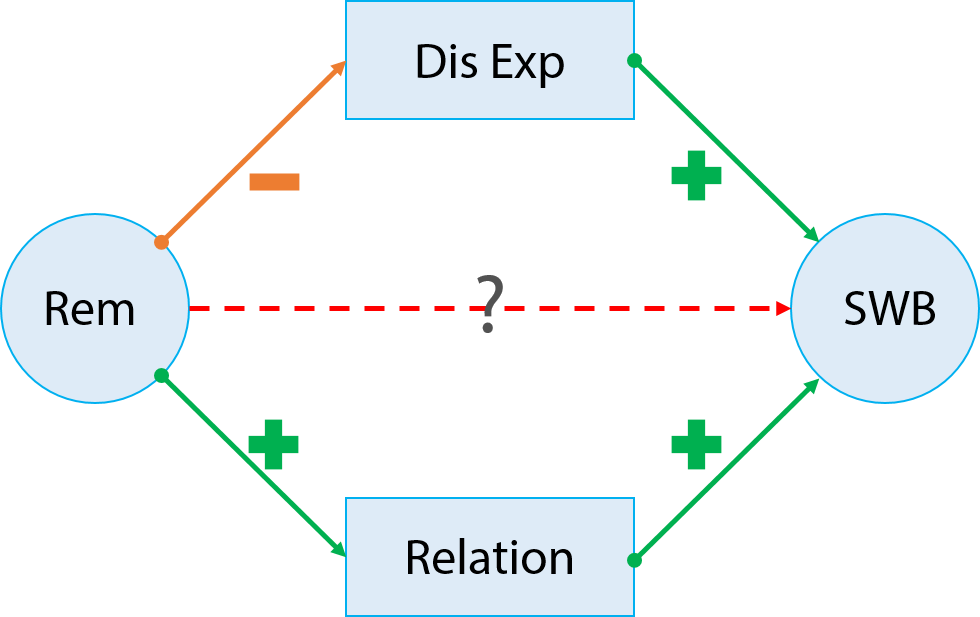
\includegraphics[width=0.52\textwidth]{mechanism.png}
\end{center}

\end{frame}



\begin{frame}[c]\frametitle{Differential Mode of Association (Fei 1947)}

\begin{itemize}
\item Relationship is a Chinese to be put in accordance with the brioche into circle from far to near, like a stone into the water to form water lines, layer by layer spread outward from a hydrophilic and hydrophobic;
\item The second is the relationship between different circles will apply different interaction law.
\item Different interpretation of altruistic and selfish
\end{itemize}
\hskip 2cm
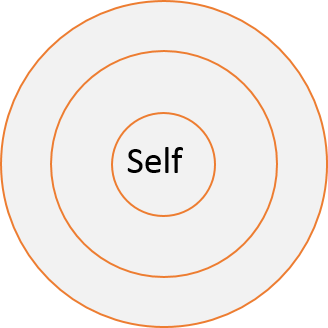
\includegraphics[width=0.23\textwidth]{order.png}

\end{frame}

\begin{frame}[c]\frametitle{Personal Utility}
\begin{itemize}
    \item Suppose the migrant maximizes his own utility with respect to the amount remitted ($r$):
\begin{equation}\label{eq:1}
    u_{m} = u\big[c_{m}(w-r),\sum_{h=1}^{n}a_{h}u(c_{h})\big] + \sum_{h=1}^{n}b_{h}V(r/n)
\end{equation}
where $w$ is the migrant\rq{}s wage, $c_{m}$ is his  consumption, $a_{h}$ are altruism weights attached to various household members, and $n$ is the household size. $b_{h}$ are the weights attached to different household memebers which measures the affinities of relationship.
\item Consumption per capita can be assumed
\begin{equation}\label{eq:2}
    c_{h} = c(y+\frac{r}{n},n)
\end{equation}
\item The migrant choose a level of $r$ to maximize \eqref{eq:1} subject to \eqref{eq:2}.
\end{itemize}
\end{frame}

\section{Data}

\begin{frame}[c]\frametitle{Data}
\begin{enumerate}
    \item Survey on Migrant Workers in Shanghai (SMWiS)-2011;
    \begin{itemize}
        \item work in Shanghai with rural registration;
        \item employee older than 16;
        \item exclude non-economic activity population (students);
        \item 1186 observations;
        \item cover the 18 counties in Shanghai;
        \item immigrate from 26 provinces;
    \end{itemize}
    \item Rural-to-urban migration in China and Indonesia(RUMiC)-2008/2009
    \begin{itemize}
        \item 8000 rural households, 5000 urban households, 5000 rural-to-urban households.
        \item 9 provinces and 15 cities;
        \item include characteristcs, education, infomation of family members left behind, expenditure in detail.
    \end{itemize}

\end{enumerate}

\end{frame}

\begin{frame}[c]\frametitle{Subjective Well-Being}
\alert{In SMWiS (2011):}
\begin{itemize}
    \item Life satisfaction index: range from 1-10;
\end{itemize}

\alert{In RUMiC (2008):}
\begin{itemize}
    \item 12 questions of the General Health Questionnaire to construct the GHQ-12 measure of mental health;
    \item GHQ-12 is one of the widely used SWB measures in economics and psychology;
    \item It is closer to being medically conventional than direct questions about “life satisfaction” or “happiness” but is highly correlated with a direct report of overall life satisfaction or happiness.
\end{itemize}
\end{frame}

\begin{frame}[c]\frametitle{Summary Statistics}

\begin{center}
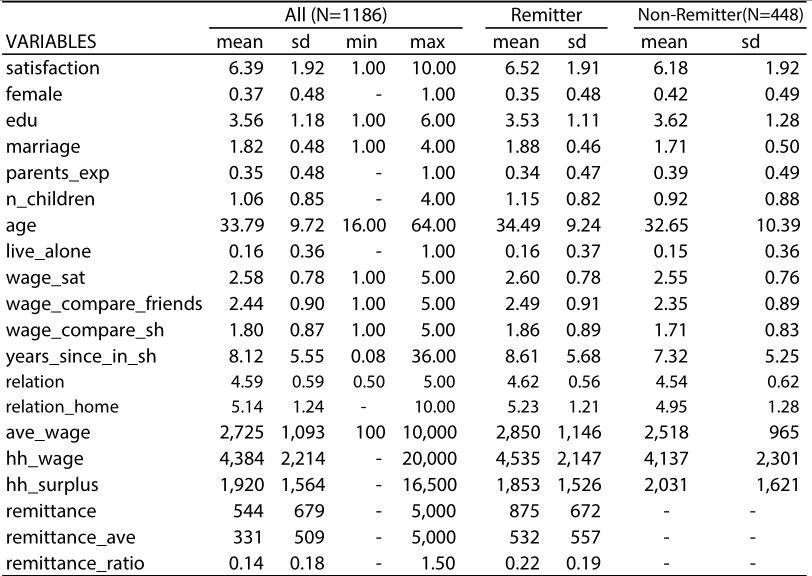
\includegraphics[width=0.9\textwidth]{summary.png}
\end{center}
\end{frame}


\begin{frame}[c]\frametitle{Life Satisfaction}
\begin{center}
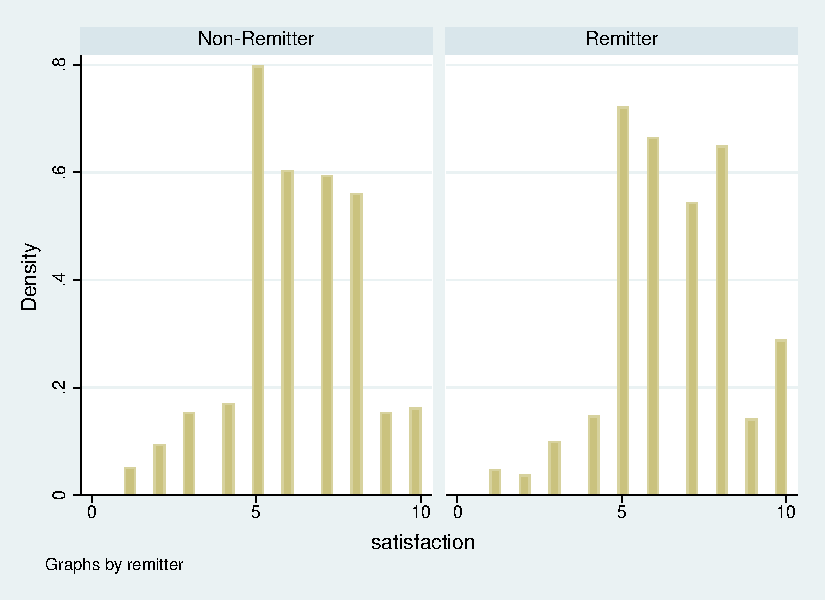
\includegraphics[width=0.9\textwidth]{satisfaction.pdf}
\end{center}
\end{frame}

\begin{frame}[c]\frametitle{Remittance}
\begin{center}
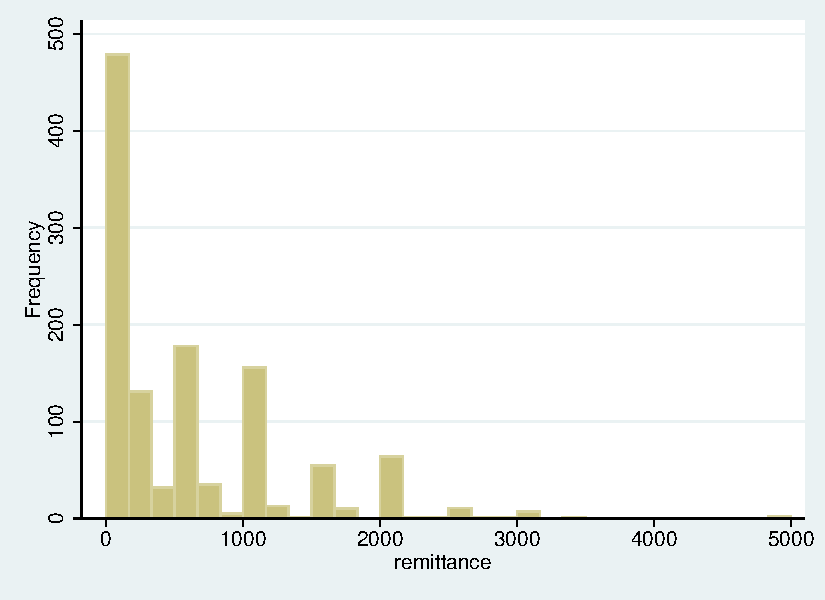
\includegraphics[width=0.9\textwidth]{remittance.pdf}
\end{center}
\end{frame}

\begin{frame}[c]\frametitle{Remittance V.S. Life Satisfaction}
\begin{center}
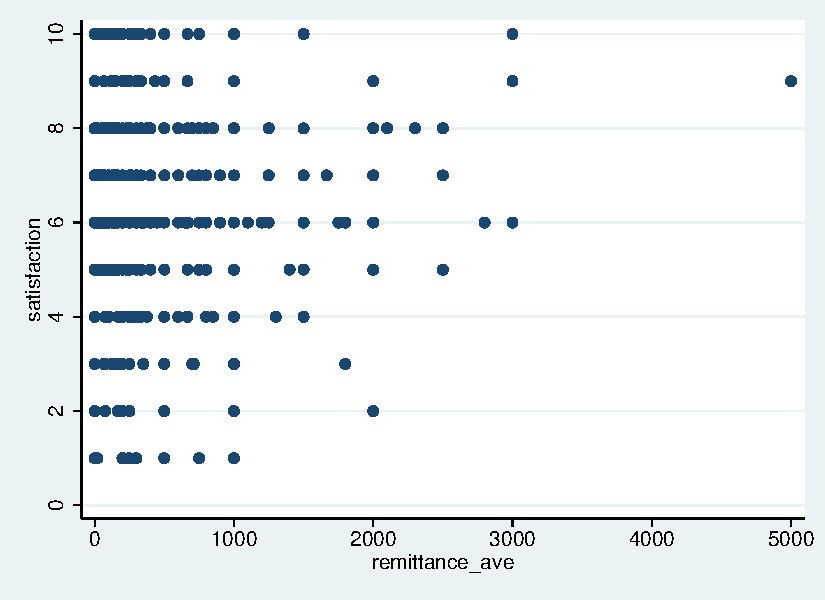
\includegraphics[width=0.9\textwidth]{satisfaction_remittance_ave.pdf}
\end{center}
\end{frame}

\begin{frame}[c]\frametitle{Remittance V.S. Relation(home)}
\begin{center}
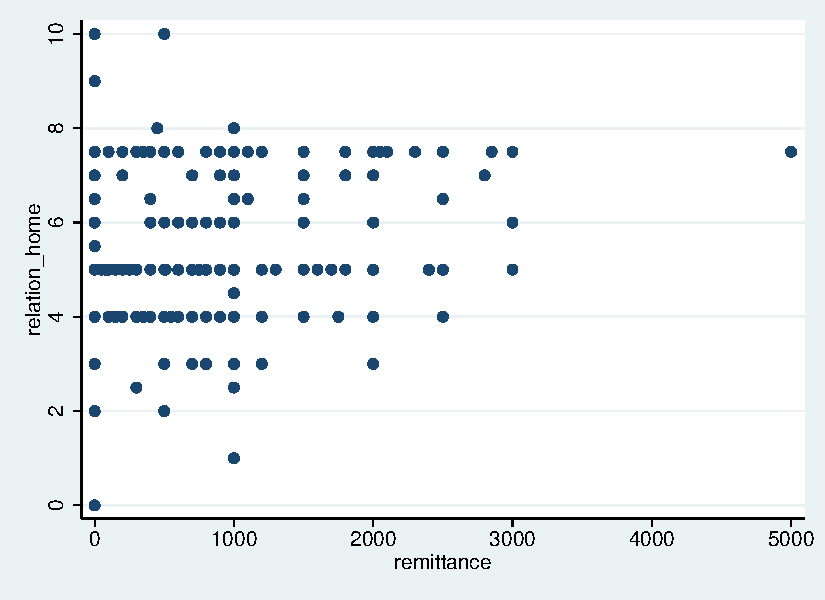
\includegraphics[width=0.9\textwidth]{relation_home_remittance.pdf}
\end{center}
\end{frame}

\section{Empirical Results}

\begin{frame}[c]\frametitle{Subjective Well-Being and Remittance}
Empirical Model:
\begin{equation}
    SWB_{ip} = \alpha + \mbf{X}_{i}\beta + \gamma r_{i} + f_{p} + \varepsilon_{i}
\end{equation}
% Table generated by Excel2LaTeX from sheet 'REG'
\begin{table}[htbp]
\scriptsize
  \centering
    \begin{tabular}{lllllll}
    \toprule
    VARIABLES & Model 1 & Model 2 & Model 3 & Model 4 & Model 5 & Model 6 \\
    \midrule
    age   & -0.015 & -0.031 & -0.024 & -0.025 & -0.024 & -0.025 \\
    age2  & 0.000 & 0.000 & 0.000 & 0.000 & 0.000 & 0.000 \\
    female & 0.237 & 0.300* & 0.365** & 0.382*** & 0.389*** & 0.389*** \\
    educated & -0.774* & -0.781* & -0.373 & -0.395 & -0.396 & -0.391 \\
    married & 0.553*** & 0.536*** & 0.547*** & 0.526*** & 0.527*** & 0.529*** \\
    live alone & -0.014 & -0.036 & 0.009 & -0.007 & -0.033 & -0.007 \\
    n\_children & -0.049 & -0.033 & -0.021 & -0.021 & -0.019 & -0.019 \\
    years\_since\_in\_sh & 0.0614*** & 0.0566*** & 0.0572*** & 0.0561*** & 0.0562*** & 0.0567*** \\
    wage\_compare\_friends &       &       & 0.483*** & 0.477*** & 0.477*** & 0.481*** \\
    wage\_compare\_sh &       &       & 0.231*** & 0.221*** & 0.221*** & 0.220*** \\
    ave\_wage &       & 0.121* & -0.022 &       &       &  \\
    remittance &       &       &       & 0.0677 &       &  \\
    remittance\_ave &       &       &       &       & 0.1120 &  \\
    remittance\_ratio &       &       &       &       &       & 0.2360 \\
    Constant & 6.350*** & 6.354*** & 4.716*** & 4.710*** & 4.697*** & 4.701*** \\
    Observations & 1,017 & 1,017 & 911   & 910   & 910   & 909 \\
    R-squared & 0.059 & 0.063 & 0.147 & 0.147 & 0.147 & 0.147 \\
    \bottomrule
    \end{tabular}%
  \label{tab:addlabel}%
\end{table}%


\end{frame}

\begin{frame}[c]\frametitle{Subjective Well-Being, Remittance and Relation}
Empirical Model:
\begin{equation}
    SWB_{ip} = \alpha + \mbf{X}_{i}\beta + \gamma r_{i} + RL_{i} + f_{p} + \varepsilon_{i}
\end{equation}
% Table generated by Excel2LaTeX from sheet 'REG2'
\begin{table}[htbp]
\scriptsize
  \centering
    \begin{tabular}{lccccc}
    \toprule
    VARIABLES & Model 1 & Model 2 & Model 3 & Model 4 & Model 5 \\
    \midrule
    age   & -0.0246 & -0.0151 & -0.0266 & -0.0178 & -0.0174 \\
    female & 0.382*** & 0.383*** & 0.355** & 0.346** & 0.350*** \\
    married & 0.526*** & 0.467*** & 0.506*** & 0.454*** & 0.442*** \\
    live\_alone & -0.00729 & 0.0307 & 0.0261 & 0.0802 & 0.0728 \\
    n\_children & -0.0207 & -0.0287 & -0.0236 & -0.0308 & -0.0324 \\
    years\_since\_in\_sh & 0.0561*** & 0.0564*** & 0.0538*** & 0.0539*** & 0.0536*** \\
    wage\_compare\_sh & 0.221*** & 0.225*** & 0.216*** & 0.223*** & 0.219*** \\
    wage\_compare\_friends & 0.477*** & 0.461*** & 0.476*** & 0.461*** & 0.459*** \\
    remittance & 0.0677 & 0.0468 & 0.0795 &       & 0.0609 \\
    relation &       & 0.380*** &       & 0.395*** & 0.392*** \\
    hh\_expenditure &       &       & 0.0611 & 0.0720* & 0.0757* \\
    Constant & 4.710*** & 2.858*** & 4.673*** & 2.749*** & 2.759*** \\
    Observations & 910   & 909   & 910   & 909   & 909 \\
    R-squared & 0.147 & 0.159 & 0.148 & 0.16  & 0.161 \\
    \bottomrule
    \end{tabular}%
\end{table}%


\end{frame}

\begin{frame}[c]\frametitle{Relation(Home) with Remittance}
Empirical Model:
\begin{equation}
    RL_{i} = \alpha + \mbf{X}_{i}^{\prime}\beta^{\prime} + \gamma^{\prime} r_{i} + f_{p}^{\prime} + \varepsilon^{\prime}_{i}
\end{equation}
% Table generated by Excel2LaTeX from sheet 'REG3'
\begin{table}[htbp]
\scriptsize
  \centering
    \begin{tabular}{lccc|ccc}
    \toprule
    Dependent Var & \multicolumn{3}{c}{Relation} & \multicolumn{3}{c}{Relation\_Home} \\
    \midrule
    Variables & Model 1 & Model 2 & Model 3 & Model 4 & Model 5 & Model 6 \\
    age   & 0.012 & 0.015 & 0.012 & 0.022 & 0.0345* & 0.030 \\
    female & -0.035 & -0.026 & -0.031 & -0.337*** & -0.270*** & -0.292*** \\
    divorced & -0.287*** & -0.322*** & -0.287*** & -0.961 & -1.818*** & -0.958 \\
    live\_alone & -0.140*** & -0.115*** & -0.150*** & 1.360*** & 1.402*** & 1.285*** \\
    n\_children & -0.011 & -0.019 & -0.011 & -0.001 & -0.030 & -0.018 \\
    family\_members\_sh & 0.003 & 0.011 & 0.011 & -0.174* & -0.132 & -0.102 \\
    years\_since\_in\_sh & -0.001 & -0.001 & -0.001 & -0.002 & -0.001 & -0.002 \\
    remittance & 0.0621*** &       &       & 0.205*** &       &  \\
    remittance\_ratio &       & 0.262*** &       &       & 1.315*** &  \\
    remittance\_ave &       &       & 0.093*** &       &       & 0.524*** \\
    Constant & 4.494*** & 4.417*** & 4.474*** & 5.784*** & 6.219*** & 5.511*** \\
    Observations & 1,162 & 1,157 & 1,162 & 745   & 742   & 745 \\
    R-squared & 0.021 & 0.023 & 0.021 & 0.282 & 0.333 & 0.308 \\
    \bottomrule
    \end{tabular}%
\end{table}%

\end{frame}

\section{Results From RUMiC 2008}
\begin{frame}[c]\frametitle{Facts From RUMiC}
\begin{center}
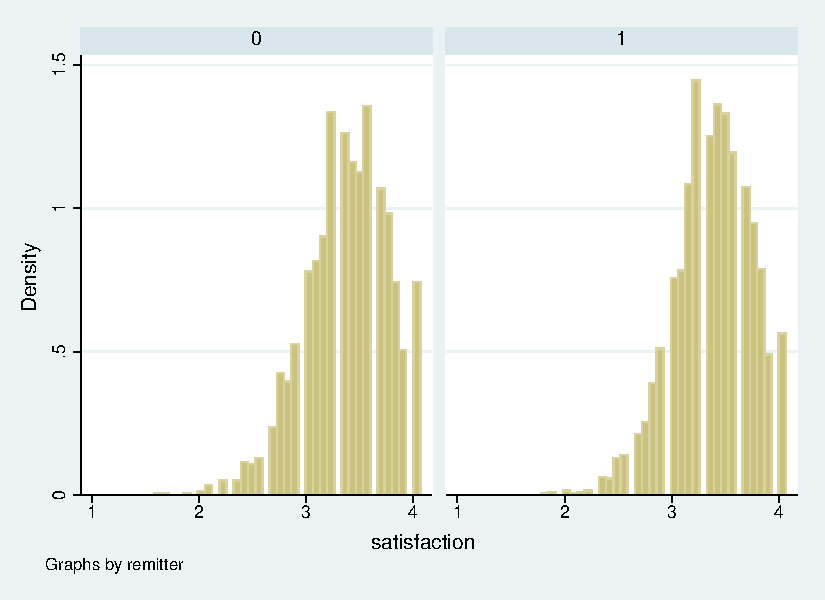
\includegraphics[width=0.9\textwidth]{satisfaction_rumic.pdf}
\end{center}
\end{frame}

\begin{frame}[c]\frametitle{Facts From RUMiC}
\begin{center}
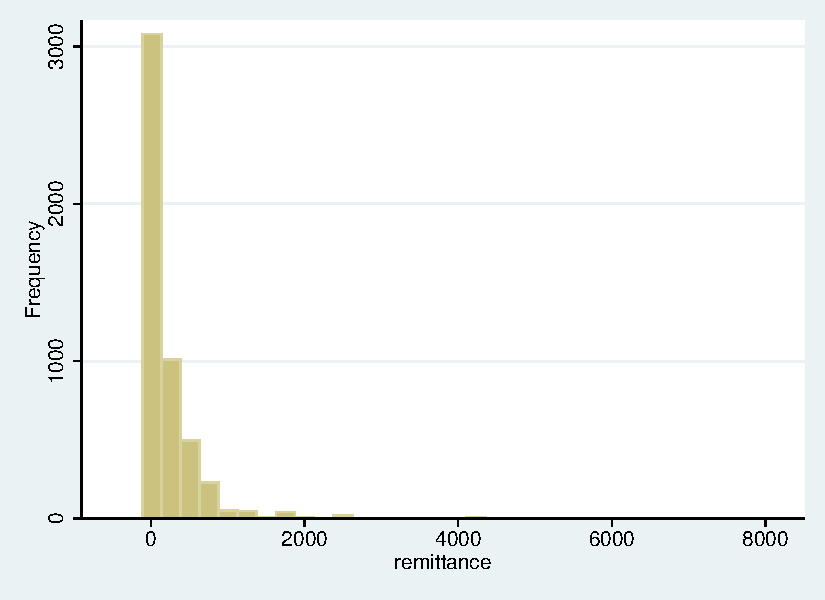
\includegraphics[width=0.9\textwidth]{remittance_rumic.pdf}
\end{center}

\end{frame}


\begin{frame}[c]\frametitle{Empirical Results}

% Table generated by Excel2LaTeX from sheet 'Sheet1'
\begin{table}[htbp]
\scriptsize
  \centering
    \begin{tabular}{lcccccc}
    \toprule
    VARIABLES & Model 1 & Model 2 & Model 3 & Model 4 & Model 5 & Model 6 \\
    \midrule
    age   & -0.0258* & -0.0261* & -0.0250* & -0.0260* & -0.0255* & -0.0239* \\
    female & -0.794*** & -0.774*** & -0.761*** & -0.780*** & -0.775*** & -0.754*** \\
    never\_married & -0.827*** & -0.786*** & -0.770*** & -0.814*** & -0.818*** & -0.634*** \\
    health & 1.802*** &       & 1.820*** & 1.804*** & 1.820*** & 1.797*** \\
    remittance &       & 0.483** & 0.529*** &       &       & 0.477** \\
    remittance\_inc\_ratio &       &       &       & 0.558 &       &  \\
    remittance\_exp\_ratio &       &       &       &       & 0.782 &  \\
    hh\_income &       &       &       &       &       & 0.117* \\
    Constant & 38.54*** & 41.77*** & 38.34*** & 38.47*** & 38.40*** & 38.04*** \\
    Observations & 4,920 & 4,920 & 4,920 & 4,912 & 4,919 & 4,920 \\
    R-squared & 0.035 & 0.017 & 0.038 & 0.036 & 0.036 & 0.040 \\
    \bottomrule
    \end{tabular}%
  \label{tab:addlabel}%
\end{table}%


\end{frame}

\section{Concerns}
\begin{frame}[c]\frametitle{Some Concerns}

\begin{enumerate}
\item How to deal with reverse causality?
\item Heterogeneity considerations, interaction terms.
\item Data problems?
\item Missing variables?
\item Does identity matters?
\item What about income inequality?
\end{enumerate}
\end{frame}

\end{document}
